% Exact LaTeX recreation of the supplied Phase-1.pdf
% Compile with pdfLaTeX. Place member pictures in the same folder if required.

\documentclass[11pt,a4paper]{article}

\usepackage[a4paper,left=2.0cm,right=2.0cm,top=1.55cm,bottom=1.55cm]{geometry}
\usepackage[T1]{fontenc}
\usepackage{lmodern}
\usepackage{graphicx}
\usepackage{xcolor}
\usepackage{array}
\usepackage{tabularx}
\usepackage{ragged2e}
\usepackage{enumitem}
\usepackage{fancyhdr}
\usepackage{tikz}
\usetikzlibrary{arrows.meta, positioning}
\usepackage{setspace}

% -------------------------------------------------
% COLOURS
% -------------------------------------------------
\definecolor{TitleBlue}{RGB}{61,103,154}

% -------------------------------------------------
% GENERAL SETTINGS
% -------------------------------------------------
\setlength{\parindent}{0pt}
\setlength{\parskip}{0pt}
\renewcommand{\arraystretch}{1.0}

% The supplied document uses a clean sans-serif heading style
% and italic serif-style explanatory text.
\newcommand{\blueheading}[1]{%
    {\sffamily\color{TitleBlue}\fontsize{15}{18}\selectfont #1}%
}

\newcommand{\bluebigheading}[1]{%
    {\sffamily\bfseries\color{TitleBlue}\fontsize{16}{19}\selectfont #1}%
}

\newcommand{\instruction}[1]{%
    {\itshape\fontsize{10.5}{12.5}\selectfont #1}%
}

\newcommand{\answerbox}[2][3.0cm]{%
    \vspace{2pt}
    \noindent
    \fbox{%
        \begin{minipage}[t][#1][t]{\dimexpr\textwidth-2\fboxsep-2\fboxrule\relax}
            \vspace{1mm}
            \itshape #2
        \end{minipage}
    }
}

% -------------------------------------------------
% HEADER / FOOTER
% -------------------------------------------------
\pagestyle{fancy}
\fancyhf{}
\renewcommand{\headrulewidth}{0pt}
\renewcommand{\footrulewidth}{0pt}

\fancyhead[L]{%
    \sffamily\bfseries\itshape\fontsize{10.5}{12}\selectfont
    Data Structure And Programming In C++ -- DSCPP
}

\fancyhead[R]{%
    \sffamily\bfseries\fontsize{10.5}{12}\selectfont
    PROJECT PROPOSAL
}

\fancyfoot[R]{%
    \itshape\fontsize{10}{12}\selectfont
    Page \thepage
}

\setlength{\headheight}{14pt}
\setlength{\headsep}{23pt}
\setlength{\footskip}{24pt}

% -------------------------------------------------
% PAGE 1
% -------------------------------------------------
\begin{document}

\vspace*{4mm}

\bluebigheading{PROJECT AND TEAM INFORMATION}

\vspace{13mm}

\blueheading{Project Title}

\vspace{1mm}

\answerbox[1.0cm]{RideSync: A Graph-Based Smart Cab Booking and Dispatch Simulation System}

\vspace{13mm}

\blueheading{Student / Team Information}

\vspace{2mm}

% Team information table
% Compact 4-member layout so all members remain on Page 1.
\noindent
\begin{tabularx}{\textwidth}{|>{\RaggedRight\arraybackslash}p{0.69\textwidth}|>{\RaggedRight\arraybackslash}X|}
\hline
\begin{minipage}[t]{\linewidth}
\vspace{1.5mm}
\textit{Team Name:}\\[-1mm]
\textit{Team ID:}
\vspace{1.5mm}
\end{minipage}
&
\begin{minipage}[t]{\linewidth}
\vspace{1.5mm}
\textit{The Four Bytes}\\[-1mm]
\textit{DSCPP-III-2026-T151}
\vspace{1.5mm}
\end{minipage}
\\
\hline
\begin{minipage}[t][3.25cm][t]{\linewidth}
\vspace{1.5mm}
\textbf{Team member 1 (Team Lead)}\\[-1mm]
\textit{(Last Name, name: student ID: email, picture):}
\vspace{2.0cm}
\end{minipage}
&
\begin{minipage}[t][3.25cm][t]{\linewidth}
\vspace{1.5mm}
\textit{Gupta, Tanvi -- 2510010362}\\
\textit{tanvigupta2005.tg@gmail.com}

\vspace{2mm}
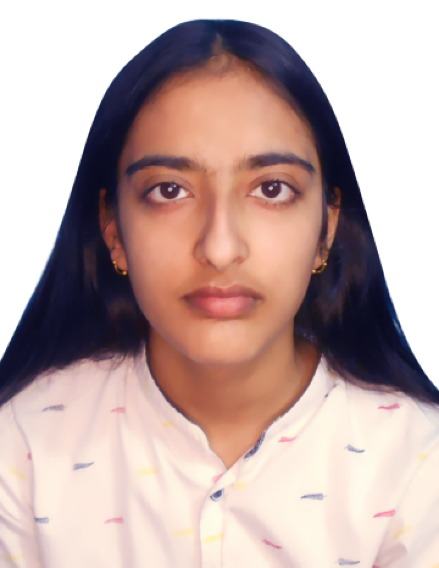
\includegraphics[width=3.0cm,height=1.5cm,keepaspectratio]{t.jpeg}
\end{minipage}
\\
\hline
\begin{minipage}[t][3.25cm][t]{\linewidth}
\vspace{1.5mm}
\textbf{Team member 2}\\[-1mm]
\textit{(Last Name, name: student ID: email, picture):}
\vspace{2.0cm}
\end{minipage}
&
\begin{minipage}[t][3.25cm][t]{\linewidth}
\vspace{1.5mm}
\textit{Jahnavi -- 2510380066}\\
\textit{jahnavimittal89@gmail.com}

\vspace{2mm}
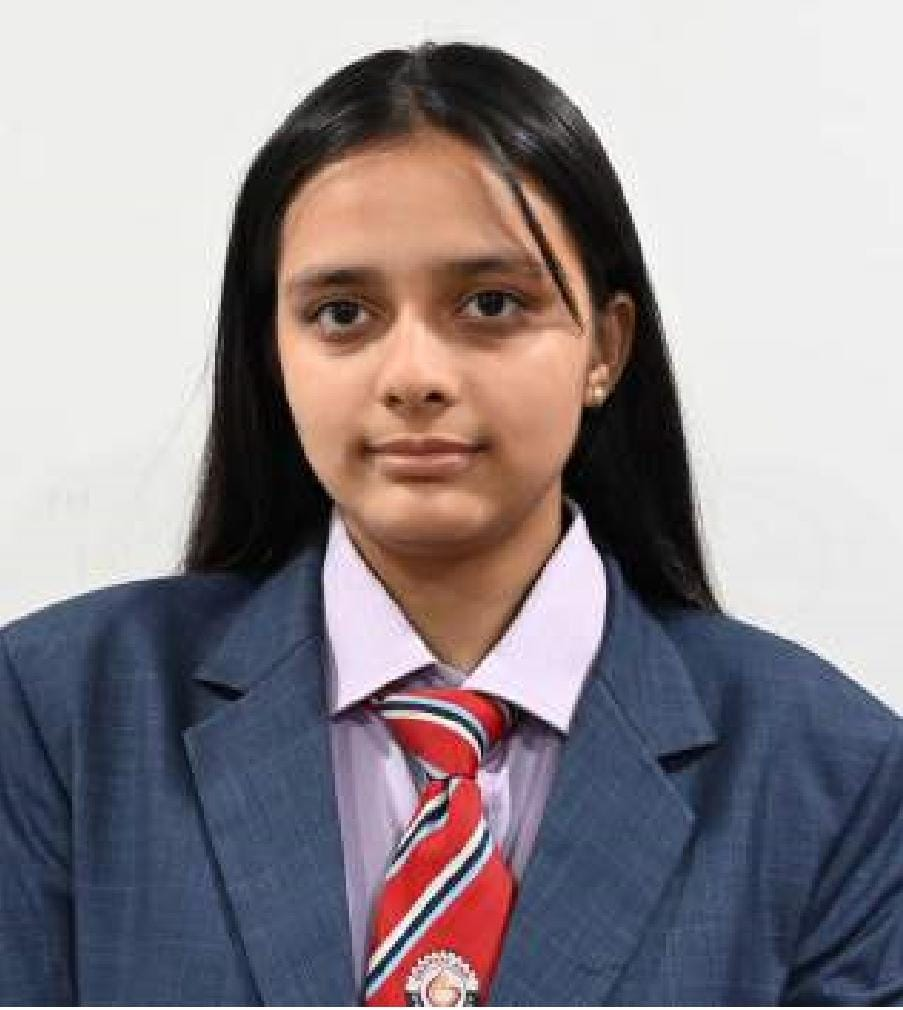
\includegraphics[width=3.0cm,height=1.5cm,keepaspectratio]{j.jpeg}
\end{minipage}
\\
\hline
\begin{minipage}[t][3.25cm][t]{\linewidth}
\vspace{1.5mm}
\textbf{Team member 3}\\[-1mm]
\textit{(Last Name, name: student ID: email, picture):}
\vspace{2.0cm}
\end{minipage}
&
\begin{minipage}[t][3.25cm][t]{\linewidth}
\vspace{1.5mm}
\textit{Tyagi, Nishtha -- 2510370096}\\
\textit{nishthatyagii29@gmail.com}

\vspace{2mm}
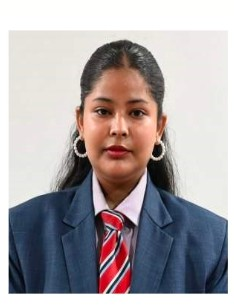
\includegraphics[width=3.0cm,height=1.5cm,keepaspectratio]{n .jpeg}
\end{minipage}
\\
\hline
\begin{minipage}[t][3.25cm][t]{\linewidth}
\vspace{1.5mm}
\textbf{Team member 4}\\[-1mm]
\textit{(Last Name, name: student ID: email, picture):}
\vspace{2.0cm}
\end{minipage}
&
\begin{minipage}[t][3.25cm][t]{\linewidth}
\vspace{1.5mm}
\textit{Sharma, Dhairya -- 2510011490}\\
\textit{sharmadhairya820@gmail.com}

\vspace{2mm}
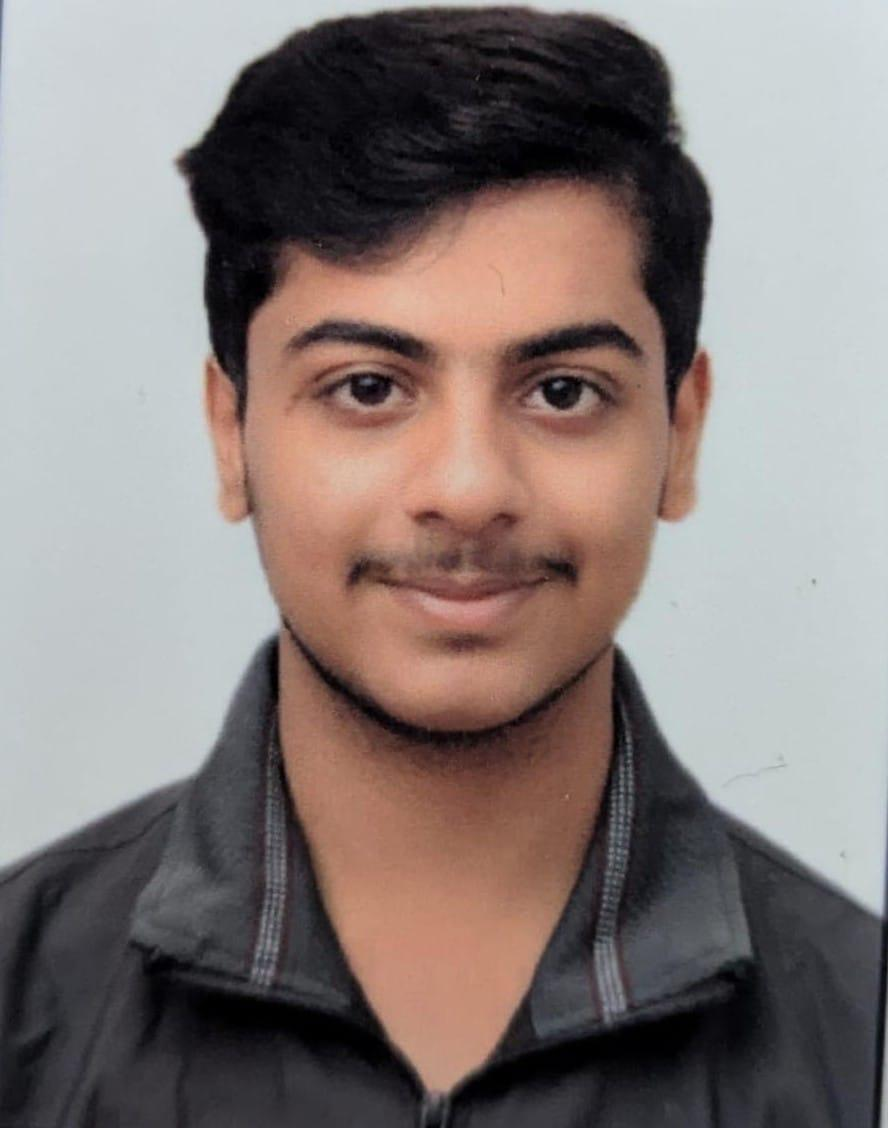
\includegraphics[width=3.0cm,height=1.5cm,keepaspectratio]{d.jpeg}
\end{minipage}
\\
\hline
\end{tabularx}

\newpage

% -------------------------------------------------
% PAGE 2
% -------------------------------------------------

\bluebigheading{PROPOSAL DESCRIPTION}

\vspace{12mm}

\blueheading{Motivation}

\vspace{1mm}

\answerbox[9.5cm]{
Booking a cab through traditional methods such as phone calls or standing at a taxi stand is inefficient and unorganised. Customers face difficulty in determining the closest cab, drivers are assigned manually without considering distance or availability, and no proper system is present in these apps to calculate the shortest path between the pickup and drop locations.Most of the times this results  in longer waiting times, random driver allocation, and inconsistent charges .

As a team, we want to explore how these real-world inefficiencies can be modelled and solved pro-grammatically using core computer science concepts.We want to build a Console-Based Cab Booking System that organises Customers, drivers and cab Data using Object Oriented Programming, represents the locations and paths as weighted graph, computes the shortest path using Dijkstra’s Algorithm, and assigns the most suitable available driver using a priority queue based on proximity and availability.

We have selected this project as our PBL exercise because it combines multiple topics from our Syllabus like data structures, algorithms, and software design  into one working project instead of treating them as distinct topics.We will implement this in C++17 because it allows us to apply  STL containers such as vector, queue, priority queue, and unordered map practically, while using fundamentals like classes, encapsulation, and modular design.File handling gives the system persistence across runs, similar to how real booking platforms retain records.

In Conclusion, this project lets us practise translating a everyday problem into a well structured programming solution, while meaningfully applying the OOP and DSA concepts covered in our current semester.
}

\vspace{12mm}

\blueheading{State of the Art / Current solution}

\vspace{1mm}

\answerbox[7cm]{
Modern cab-booking platforms such as Uber and Ola solve this problem using large-scale, GPS-enabled infrastructure. When a customer looks for a cab to book a ride ,Program look at the live location of the customer to find availability of nearby drivers, apply algorithm that looks at the distance, driver rating, and demand, and calculates the shortest path using real-time mapping services.

On the basis of  distance, traffic, and demand,the fare is calculated and a permanent record is maintained on the server that stores the transaction, including the payment made by the customer. These systems use components that are theoretically same to what we plan on building i.e. driver matching, shortest-path calculation, and fare calculation – but at a scale involving  dynamic location  services, distributed servers, and payment gateways that are far beyond the scope of current time period provided for the PBL.

Our project focuses on the existing algorithmic and data-structure problems behind such platforms rather than copying their infrastructure.We simulate locations, roads, and driver positions using already defined data instead of GPS, and concentrate on correctly implementing graph based routing, priority based driver assignment, and modular OOPs design in C++17.
}

\vspace{12mm}
\newpage
\blueheading{Project Goals and Milestones}

\vspace{1mm}

\answerbox[10 cm]{
Our primary goal is to design and implement a modular, console-based Cab Booking System in C++17 that demonstrates meaningful use of Object-Oriented Programming and core Data Structures and Algorithms, while remaining realistically achievable by a team of four third-semester students.

Specific goals: build separate, well-encapsulated modules for Customer, Driver, Admin, and Booking management; represent the city's locations and roads as a weighted graph and compute shortest routes using Dijkstra's Algorithm; assign the most suitable available driver using a priority queue; estimate fares based on computed distance; and persist customer, driver, cab, and booking data using file handling so information is retained between runs.

Planned milestones:

\textit{Phase 1 (Weeks 1--2):} Problem definition, requirement analysis, and overall system design.

\textit{Phase 2 (Weeks 3--4):} Design of the class structure and modules; implementation of the authentication manager and basic customer/driver/admin modules.

\textit{Phase 3 (Weeks 5 to  6):} Implementation of the graph that represents location ,  Dijkstra’s algorithm that calculates the shortest route and driver assessment based on priority queue.


\textit{Phase 4 (Weeks 7 to  8):} Implementation of the booking system , calculation of fare and persistence of all modules on the basis of stored data.

\textit{Phase 5 (Weeks 9 to  10):} Integration of allmodules, testing, debugging, documentation, and  final demonstration.

This plan lets us work on the project evenly by dividing the work equally among each member . For example two members focus on the booking module and the other two focus on the graphn and priority queue based booking algorithms and then we can integrate each part.
}

\vspace{12mm}

\blueheading{Project Approach}

\vspace{1mm}

\answerbox[7cm]{
\fontsize{9.5}{11.5}\selectfont

Our implementation depends on C++17 and standard OOPs principles. We are breaking the system into various classes—Customer, Driver, Cab, Admin, and Booking ensuring data stays properly encapsulated with private properties and clean public interfaces. An Authentication Manager handles user logins, while Booking Manager acts as the central controller to wire up routing, fare calculations, and assigning the drivers.

For the underlying map, we're representing city locations and road connections using an
adjacency list via \texttt{std::unordered\_map<int, std::vector<std::pair<int, int>>>}.
Shortest path and distance calculations between pickup and drop-off points run through
Dijkstra's Algorithm, powered by \texttt{std::priority\_queue}. A second priority queue
ranks available nearby drivers using a composite score of distance and overall rating to
assign the best match quickly.

Rather than reinventing standard data structures, we make heavy use of the Standard Template Library (vector, queue, priority queue, unordered map, and a stack for recent booking history), keeping our focus on core business logic. Persistence is straightforward: user and booking records save directly to flat text files between runs.

Each module lives in its own dedicated header/source pair for clean separation, and we've added input validation (handling things like bad location IDs or out-of-service cabs) to keep the terminal interface from crashing. The team consists of four members collaborating via GitHub and working out of VS Code, with a focus on unit testing each module before putting everything together.
}
\newpage

% -------------------------------------------------
% PAGE 3
% -------------------------------------------------
\blueheading{System Architecture (High Level Diagram)}

\vspace{1mm}

\answerbox[5.0cm]{
    \centering
    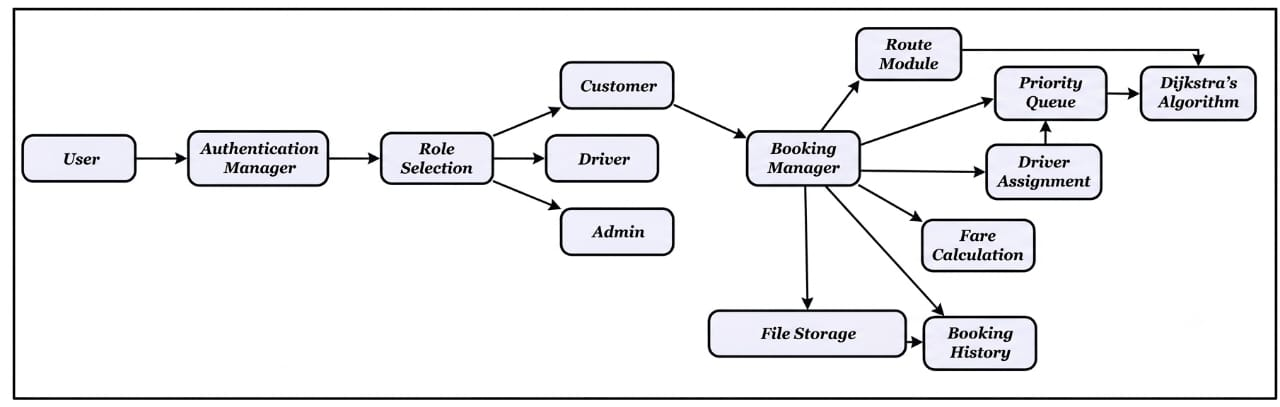
\includegraphics[width=15cm\textwidth,height=7cm,keepaspectratio]{flowchart.jpeg}
}

\vspace{12mm}

\blueheading{Project Outcome / Deliverables}

\vspace{1mm}

\answerbox[7cm]{
By the end of this project, we expect to deliver a fully working, console-based Cab Booking System implemented in C++17, including: a Customer module supporting registration, login, cab booking, and booking history; a Driver module supporting registration, login, and availability management; an Admin module for managing cabs, drivers, and viewing basic statistics; a graph-based route module that computes the shortest path between pickup and destination using Dijkstra's Algorithm; a priority-queue-based driver assignment mechanism that selects the most suitable available driver; a fare-calculation module based on the computed route distance; file-based persistence for customer, driver, cab, and booking data across program executions; booking history and cancellation handling for customers; a short project report with basic testing documentation; and a GitHub repository containing the complete, organised source code with commit history reflecting each team member's contribution.
}

\vspace{12mm}

\blueheading{Assumptions}

\vspace{6mm}

\answerbox[3cm]{
All locations defined in the program are predefined and stored internally as graph vertices; the system does not use live GPS data. Distances/road weights between locations are predefined and fixed for the simulation. Payments are simulated and no real payment gateway is integrated. Drivers, cabs, and their availability status are represented using data stored and updated by the program, not by live tracking. The system runs through a console (text-based) interface only. No network connectivity or external API access is required; all data is stored and read locally using files.
}

\vspace{12mm}
\newpage
\blueheading{References}

\vspace{1mm}

\answerbox[5cm]{
\begin{itemize}[leftmargin=4mm, itemsep=1pt, topsep=1pt]
\item cppreference.com -- C++17 Language and Standard Library Reference, \url{https://en.cppreference.com/}
\item GeeksforGeeks -- Object-Oriented Programming in C++, \url{https://www.geeksforgeeks.org/object-oriented-programming-in-cpp/}
\item GeeksforGeeks -- Dijkstra's Shortest Path Algorithm, \url{https://www.geeksforgeeks.org/dijkstras-shortest-path-algorithm-greedy-algo-7/}
\item cplusplus.com -- C++ STL Containers Reference, \url{https://cplusplus.com/reference/stl/}
\item cplusplus.com -- File Handling in C++ (fstream), \url{https://cplusplus.com/doc/tutorial/files/}
\end{itemize}
}

\end{document}